\documentclass[11pt,a4paper]{article}

\usepackage[T1]{fontenc}
\usepackage[utf8]{inputenc}
\usepackage{lmodern}
\usepackage[a4paper,margin=1in]{geometry}
\usepackage{microtype}
\usepackage{setspace}
\usepackage{booktabs}
\usepackage{tabularx}
\usepackage{longtable}
\usepackage{array}
\usepackage{enumitem}
\usepackage{amsmath}
\usepackage{amssymb}
\usepackage{float}
\usepackage{graphicx}
\usepackage{xcolor}
\usepackage{hyperref}
\usepackage{fancyhdr}
\usepackage{titlesec}
\usepackage{tikz}
\usepackage{pgfplots}
\usetikzlibrary{arrows.meta,positioning,shapes.geometric,fit,backgrounds}
\pgfplotsset{compat=1.18}

\hypersetup{
  colorlinks=true,
  linkcolor=black,
  urlcolor=blue!50!black,
  citecolor=black
}

\definecolor{accent}{HTML}{163A5F}
\definecolor{softaccent}{HTML}{EAF1F7}
\definecolor{lightborder}{HTML}{D7E0EA}
\definecolor{softgray}{HTML}{F6F7F9}

\titleformat{\section}{\large\bfseries\color{accent}}{\thesection.}{0.6em}{}
\titleformat{\subsection}{\normalsize\bfseries\color{accent}}{\thesubsection}{0.6em}{}
\titleformat{\subsubsection}{\normalsize\bfseries}{\thesubsubsection}{0.6em}{}

\setlength{\parindent}{0pt}
\setlength{\parskip}{0.65em}
\setlist[itemize]{leftmargin=1.5em}

\pagestyle{fancy}
\fancyhf{}
\fancyhead[L]{Indian Equities Market Surveillance and Contagion Platform}
\fancyhead[R]{Final Report}
\fancyfoot[C]{\thepage}

\newcolumntype{Y}{>{\raggedright\arraybackslash}X}
\newcolumntype{L}[1]{>{\raggedright\arraybackslash}p{#1}}

\begin{document}
\begin{titlepage}
    \centering
    \vspace*{1.5cm}

    {\Large \textbf{Birla Institute of Technology and Science, Pilani}\par}
    \vspace{0.4cm}
    {\large M.E. Software Systems\par}
    \vspace{1.7cm}

    {\Huge \textbf{Indian Equities Market Surveillance and Contagion Platform}\par}
    \vspace{0.6cm}
    {\Large Final Project Report\par}
    \vspace{1.2cm}

    {\large Course: \textbf{CS/SS G516 -- Advanced Database Systems}\par}
    \vspace{1.5cm}

    \begin{tabular}{ll}
        \textbf{Submitted by:} & Aryan Srivastava \\
                               & Harshvardhan Singh Kumain \\
                               & Tathya Sethi \\
                               & Ansh \\
    \end{tabular}

    \vfill

    {\large April 2026\par}
\end{titlepage}

\onehalfspacing

\begin{abstract}
This report presents a distributed market surveillance platform built for Indian equities. The project was motivated by a practical systems question: how should one design a database-backed application that must serve two very different kinds of work at the same time? On the one hand, an operator needs fast intraday monitoring, timely anomaly alerts, and a clear view of sector-level contagion. On the other, an analyst needs a clean historical store that supports trend analysis, roll-ups, drill-downs, and report generation. A single database is a poor fit for both jobs. Our answer was a layered architecture that treats the streaming path and the analytical path as separate concerns, then joins them through a controlled ETL process.

The implemented system uses Kafka as a replayable ingestion log, Cassandra as the operational time-series store, Redis as the hot-state and read-model layer, PostgreSQL for operational event persistence and warehouse analytics, Python services for collection and statistical processing, and a Next.js/FastAPI application for user interaction. The project runs in a strict real-data-only mode. At the time of writing, the platform tracks 2,388 listed symbols in its reference universe, maintains real daily history for 2,383 of them, and actively monitors a ranked intraday universe of 500 significant stocks using a captured real market session. The current materialized footprint is 1,080,064 rows across streaming, operational, and warehouse stores; at the present 500-symbol intraday scope, the design projects to 93.75 million tick-plus-anomaly rows per year.

The system is not a trading engine and does not attempt to forecast future prices. Its purpose is surveillance: detect statistically unusual movements, identify sector spillover, persist those events in forms suited to both operations and analytics, and make the result understandable to a human user. The report explains the domain, architecture, database design, implementation details, analytical query support, current scale, and a defensible final demo path.
\end{abstract}

\tableofcontents
\newpage

\section{Introduction and Project Scope}
The project addresses a familiar problem in market systems: operational workloads and analytical workloads rarely behave alike. Minute-by-minute market bars arrive in a write-heavy, append-oriented stream. Alerts must be computed while the feed is moving. At the same time, historical analysis demands carefully structured facts, dimensions, aggregate views, and user-friendly reporting. If both concerns are forced into one storage model, one of them usually suffers.

Our application is intended for the domain of Indian equity market surveillance. It is designed for two classes of users. The first is the operator, who needs a live console showing the current tape, flagged names, alert queues, and sector contagion. The second is the analyst, who needs a consolidated historical layer for cross-session analysis, signal persistence studies, sector comparisons, and report generation. Those two user stories define the scope of the project.

The implemented scope is intentionally narrower than ``the entire exchange in full intraday depth forever,'' because the current provider setup must remain real-data-only and defensible. The platform therefore separates three levels of coverage:
\begin{itemize}
    \item a \textbf{listed symbol universe} used for metadata, directory search, and reference management;
    \item a \textbf{daily history universe} used for per-stock history and longer-range indicators;
    \item a \textbf{ranked intraday universe} used for minute-level surveillance and real-time analytics.
\end{itemize}

As of 23 April 2026, the system tracks 2,388 listed symbols, hydrates daily history for 2,383 of them, and monitors 500 significant names at intraday resolution. That distinction matters. It lets the application represent the exchange broadly without claiming minute-level coverage that is not currently materialized.

Equally important is what the project does \emph{not} claim. It is not a trading platform, not a portfolio manager, not a predictive machine-learning model, and not a synthetic market simulator. The system only ingests or replays real market data. The replay mode is built from captured real sessions rather than generated fixtures. This decision keeps the presentation honest and gives every chart, anomaly, and warehouse record a traceable provenance.

\section{Final Feature Set and Application Domain}
The application serves the market surveillance domain, where the goal is to notice unusual market behavior early, place it in context, and preserve it in forms that are useful both intraday and after market close. Within that domain, the final feature set is as follows.

\subsection{Operational Features}
\begin{itemize}
    \item Real-data ingestion through a configurable provider layer, currently operating with \texttt{yfinance} and a strict real-data-only policy.
    \item Real captured-session replay, allowing the full stack to be demonstrated outside market hours without synthetic data.
    \item Kafka-backed streaming so raw market bars can be consumed independently by storage and analytics services.
    \item Intraday anomaly detection using EWMA-based price and volume scoring with a 20-minute warm-up guard.
    \item Sector-based contagion detection using a 5-minute observation window and deduplication per trigger symbol.
    \item Open alert management with acknowledgement support.
    \item A live operator console with overview, stock workspaces, contagion views, methodology notes, process documentation, replay status, and system health.
\end{itemize}

\subsection{Analytical Features}
\begin{itemize}
    \item A PostgreSQL warehouse with explicit dimensions, fact tables, and materialized views.
    \item Daily and intraday historical analysis for the monitored universe.
    \item Sector regime summaries, stock persistence summaries, intraday pressure profiles, and stock leaderboards.
    \item An analyst workbench with a controlled visual query builder over curated warehouse datasets.
    \item CSV export and browser-native PDF report generation through the analyst interface.
\end{itemize}

\subsection{Current System Snapshot}
\begin{table}[H]
\centering
\caption{Live system snapshot used in this report (23 April 2026)}
\begin{tabularx}{\textwidth}{L{0.48\textwidth}Y}
\toprule
\textbf{Metric} & \textbf{Value} \\
\midrule
Listed symbols in reference universe & 2,388 \\
Hydrated symbols with daily history & 2,383 \\
Intraday symbols currently loaded & 500 \\
Current intraday trading days loaded & 1 (\texttt{2026-04-22}) \\
Materialized total rows across stores & 1,080,064 \\
Streaming market ticks & 185,186 \\
Streaming anomaly metrics & 182,686 \\
Warehouse anomaly-minute rows & 182,686 \\
Warehouse contagion-event rows & 9,137 \\
Warehouse coverage rows & 185,186 \\
Tick-plus-anomaly annual projection at current scope & 93,750,000 rows \\
Real-data policy & Strict real-data-only \\
Active provider configuration & \texttt{yfinance} (\texttt{Upstox} adapter present, not configured) \\
\bottomrule
\end{tabularx}
\end{table}

\section{Architecture Overview}
The system uses polyglot persistence because the workload demands it. Kafka provides a replayable transport layer. Cassandra is used for append-heavy operational facts where partition-oriented reads matter more than relational joins. Redis holds state that must survive process restarts and also acts as the hot read model for the operator console. PostgreSQL is used twice: first as an operational relational store for contagion events, alerts, profiles, and ETL bookkeeping; second as the analytical warehouse where dimensions, facts, and materialized views live.

\begin{figure}[H]
\centering
\resizebox{0.92\textwidth}{!}{%
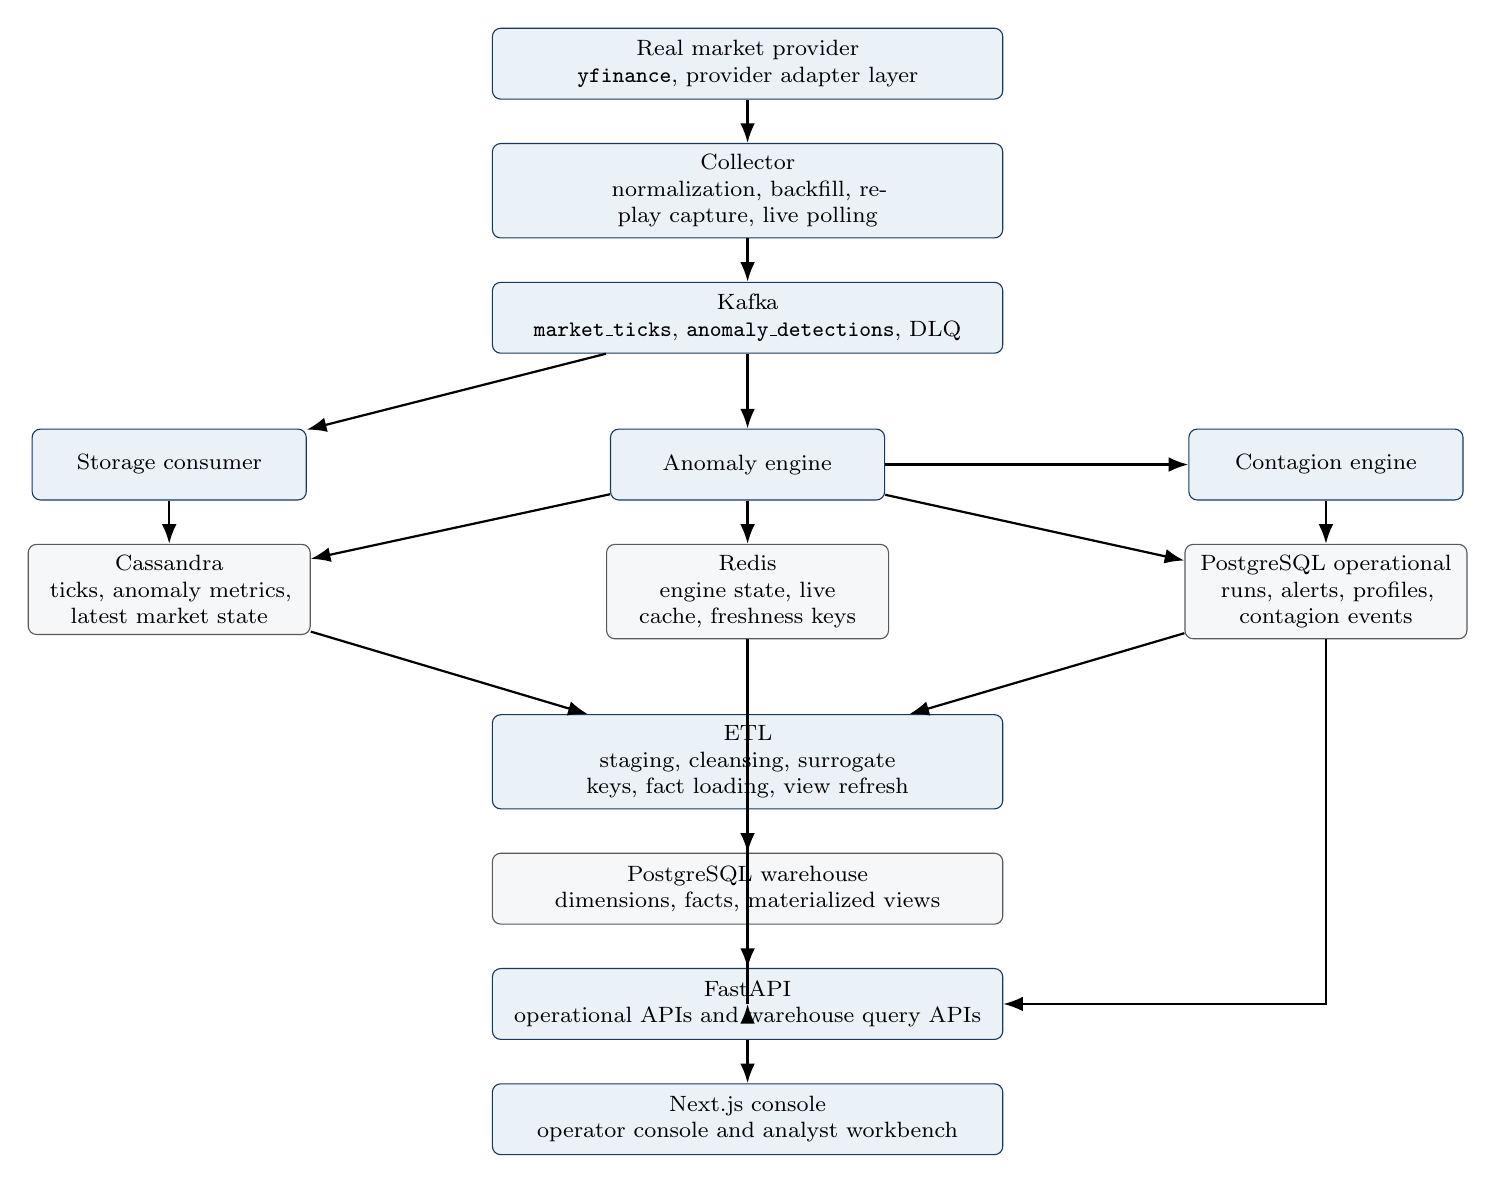
\begin{tikzpicture}[
    node distance=0.55cm and 0.6cm,
    font=\footnotesize,
    box/.style={draw=accent, rounded corners=3pt, fill=softaccent, text width=3.2cm, minimum height=0.9cm, align=center, inner sep=4pt},
    widebox/.style={draw=accent, rounded corners=3pt, fill=softaccent, text width=6.2cm, minimum height=0.9cm, align=center, inner sep=4pt},
    store/.style={draw=black!65, rounded corners=3pt, fill=softgray, text width=3.3cm, minimum height=0.9cm, align=center, inner sep=4pt},
    widestore/.style={draw=black!65, rounded corners=3pt, fill=softgray, text width=6.2cm, minimum height=0.9cm, align=center, inner sep=4pt},
    arrow/.style={-{Latex[length=2.5mm]}, thick}
]
\node[widebox] (provider) {Real market provider \\ \texttt{yfinance}, provider adapter layer};
\node[widebox, below=of provider] (collector) {Collector \\ normalization, backfill, replay capture, live polling};
\node[widebox, below=of collector] (kafka) {Kafka \\ \texttt{market\_ticks}, \texttt{anomaly\_detections}, DLQ};

\node[box, below left=0.95cm and 2.35cm of kafka] (storage) {Storage consumer};
\node[box, below=0.95cm of kafka] (anomaly) {Anomaly engine};
\node[box, below right=0.95cm and 2.35cm of kafka] (contagion) {Contagion engine};

\node[store, below=of storage] (cass) {Cassandra \\ ticks, anomaly metrics, latest market state};
\node[store, below=of anomaly] (redis) {Redis \\ engine state, live cache, freshness keys};
\node[store, below=of contagion] (pgop) {PostgreSQL operational \\ runs, alerts, profiles, contagion events};

\node[widebox, below=0.95cm of redis] (etl) {ETL \\ staging, cleansing, surrogate keys, fact loading, view refresh};
\node[widestore, below=of etl] (warehouse) {PostgreSQL warehouse \\ dimensions, facts, materialized views};
\node[widebox, below=of warehouse] (api) {FastAPI \\ operational APIs and warehouse query APIs};
\node[widebox, below=of api] (frontend) {Next.js console \\ operator console and analyst workbench};

\draw[arrow] (provider) -- (collector);
\draw[arrow] (collector) -- (kafka);
\draw[arrow] (kafka) -- (storage);
\draw[arrow] (kafka) -- (anomaly);
\draw[arrow] (anomaly) -- (contagion);
\draw[arrow] (storage) -- (cass);
\draw[arrow] (anomaly) -- (cass);
\draw[arrow] (anomaly) -- (redis);
\draw[arrow] (anomaly) -- (pgop);
\draw[arrow] (contagion) -- (pgop);
\draw[arrow] (cass) -- (etl);
\draw[arrow] (pgop) -- (etl);
\draw[arrow] (etl) -- (warehouse);
\draw[arrow] (redis) |- (api);
\draw[arrow] (pgop) |- (api);
\draw[arrow] (warehouse) -- (api);
\draw[arrow] (api) -- (frontend);
\end{tikzpicture}
}
\caption{High-level system architecture}
\label{fig:architecture}
\end{figure}

This separation is also how the project applies the central ideas from the data warehousing material used in the course. The warehouse is subject-oriented, because it is organized around stocks, sectors, dates, times, and contagion events rather than around application screens. It is integrated, because source-specific forms are normalized before loading. It is time-variant, because every fact is keyed by date and, where necessary, time. It is non-volatile in the analytical sense, because warehouse facts are loaded through ETL and then queried for analysis rather than updated continuously by business transactions.

\section{End-to-End Data Flow}
The easiest way to understand the application is to follow one market bar from source to analysis.

\begin{figure}[htbp]
\centering
\resizebox{0.94\textwidth}{!}{%
\begin{tikzpicture}[
    node distance=0.18cm,
    font=\footnotesize,
    step/.style={draw=black!60, rounded corners=3pt, fill=softgray, text width=13.1cm, align=left, inner sep=5pt},
    arrow/.style={-{Latex[length=2.2mm]}, thick}
]
\node[step] (s1) {\textbf{1. Collection and normalization.} The collector downloads bars, converts timestamps to UTC and IST, adds exchange and sector metadata, assigns a deterministic dedupe key, and emits a canonical \texttt{MarketTick}.};
\node[step, below=of s1] (s2) {\textbf{2. Kafka publication.} The normalized tick is published to Kafka with the symbol as the message key so that per-symbol ordering is preserved.};
\node[step, below=of s2] (s3) {\textbf{3. Dual consumption.} One consumer persists the raw tick to Cassandra. In parallel, the anomaly engine pulls the same tick and updates streaming statistics.};
\node[step, below=of s3] (s4) {\textbf{4. Streaming scoring.} After the warm-up period, the anomaly engine computes return percentage, EWMA mean and variance, price \(z\)-score, volume \(z\)-score, rolling volatility, and the composite score.};
\node[step, below=of s4] (s5) {\textbf{5. Hot-state persistence.} The anomaly engine writes the metric to Cassandra, refreshes Redis live state, records surveillance coverage in PostgreSQL, and emits anomaly detections to Kafka.};
\node[step, below=of s5] (s6) {\textbf{6. Contagion evaluation.} The contagion engine opens a five-minute observation window, tracks anomalous sector peers, and writes one finalized contagion event to PostgreSQL.};
\node[step, below=of s6] (s7) {\textbf{7. End-of-day ETL.} The ETL service extracts anomaly metrics for a trading date, loads staging, derives contagion flags, assigns surrogate keys, loads warehouse facts, and refreshes analytical views.};
\node[step, below=of s7] (s8) {\textbf{8. User-facing analytics.} FastAPI serves live operational views from Redis/PostgreSQL and historical analysis from the warehouse, while the frontend exposes both operator and analyst workflows.};
\draw[arrow] (s1) -- (s2);
\draw[arrow] (s2) -- (s3);
\draw[arrow] (s3) -- (s4);
\draw[arrow] (s4) -- (s5);
\draw[arrow] (s5) -- (s6);
\draw[arrow] (s6) -- (s7);
\draw[arrow] (s7) -- (s8);
\end{tikzpicture}
}
\caption{The data journey from ingestion to analytics}
\label{fig:dataflow}
\end{figure}

\subsection{Where Ingestion Happens}
The ingestion entry point is the collector service. In the code base, the normalization logic is in \path{services/collector/src/collector/main.py}, specifically the function \path{normalize_frame}. Daily history hydration is handled in the same file by \path{hydrate_daily}, captured replay creation by \path{capture_replay}, and intraday backfill by \path{backfill}. The shared provider abstraction lives in \path{shared/contracts/src/market_surveillance/market_data.py}. This file decides whether the current runtime uses \texttt{yfinance} or the optional \texttt{Upstox} adapter.

\subsection{Where Real-Time Analytics Happens}
The anomaly engine is the decision point for live signals. The core scoring function is \path{score_tick} in \path{services/anomaly-engine/src/anomaly_engine/main.py}. For a tick with close price \(P_t\) and previous close \(P_{t-1}\), the engine computes
\[
\text{return\_pct}_t = \left(\frac{P_t - P_{t-1}}{P_{t-1}}\right) \times 100.
\]
It then updates exponentially weighted mean and variance for both returns and volume. The signal terms are:
\[
\text{price\_z} = \frac{\text{return\_pct}_t - \mu_r}{\sigma_r},
\qquad
\text{volume\_z} = \frac{V_t - \mu_v}{\sigma_v},
\]
where \(\mu_r,\sigma_r\) are the EWMA return mean and standard deviation, and \(\mu_v,\sigma_v\) are the EWMA volume mean and standard deviation. The composite score is
\[
\text{composite} = 0.6 \cdot |\text{price\_z}| + 0.4 \cdot |\text{volume\_z}|.
\]
The configured thresholds are taken from \path{shared/contracts/src/market_surveillance/settings.py}: price \(z \geq 2.4\), volume \(z \geq 2.0\), composite score \(\geq 2.2\), with a 20-minute warm-up guard.

The contagion engine, implemented in \path{services/contagion-engine/src/contagion_engine/main.py}, listens only to anomaly detections rather than raw ticks. It opens a five-minute observation window for the first anomalous event in a symbol, ignores duplicate triggers for the same symbol while that window is active, and tracks peer anomalies in the same sector. When the window closes, it computes
\[
\text{risk score} = \text{trigger score} + \text{peer average score} + 0.35 \times \text{affected count},
\]
then writes one relational event to PostgreSQL.

\section{Database Design}
The database design is the core of the project. The design is not just a list of technologies; it is the answer to a set of workload questions.

\subsection{Kafka as the Replayable Ingestion Log}
Kafka sits between collection and downstream processing because it decouples the arrival of raw bars from the speed of consumers. The collector publishes normalized ticks to \texttt{market\_ticks}. Storage and anomaly scoring consume the same stream independently. A malformed payload can be routed to the dead-letter topic without stopping the pipeline. Replay is possible because Kafka is treated as a commit log rather than a fire-and-forget transport.

\subsection{Cassandra as the Operational Time-Series Store}
The Cassandra schema is query-driven. The table definitions in \path{infra/cassandra/schema.cql} are designed for append-heavy writes and per-symbol, per-day time-range access:
\begin{itemize}
    \item \texttt{market\_ticks} stores normalized raw bars, partitioned by \((\texttt{symbol}, \texttt{trading\_date})\) and clustered by \texttt{timestamp\_utc}.
    \item \texttt{anomaly\_metrics} stores the per-minute anomaly output with the same partition design.
    \item \texttt{latest\_market\_state} provides a direct latest-value lookup for each monitored symbol.
\end{itemize}

This is a good match for the streaming layer because the write pattern is append-oriented and the principal reads are bounded time slices within a symbol and a trading date. Cassandra is not exposed as the main analytical interface. Human-facing analytical work is delegated to PostgreSQL.

\subsection{Redis as the State and Hot-Read Layer}
Redis plays two roles. First, it stores restart-critical anomaly state: the EWMA statistics needed to continue scoring without rebuilding the full recent window from Cassandra. Second, it stores the latest live read models for the UI, such as the latest market snapshot and latest anomaly per symbol. This design keeps the frontend from repeatedly hitting Cassandra for hot reads and keeps restart behavior predictable.

\subsection{PostgreSQL Operational Schema}
PostgreSQL has an operational schema that stores the parts of the system that are relational by nature or operationally important:
\begin{itemize}
    \item \texttt{operational.ingestion\_runs} records collection, replay, and backfill runs.
    \item \texttt{operational.etl\_runs} records extraction and warehouse load metadata.
    \item \texttt{operational.surveillance\_coverage} records that a symbol was under monitoring even during warm-up.
    \item \texttt{operational.contagion\_events} stores finalized contagion events.
    \item \texttt{operational.stock\_profiles}, \texttt{stock\_daily\_bars}, and \texttt{alert\_events} support the UI and system operations.
\end{itemize}

This layer matters for the viva because it shows that the project distinguishes between operational truth and analytical truth. Not every relational table belongs in the warehouse; some belong to the live system itself.

\subsection{PostgreSQL Warehouse Schema}
The warehouse schema is defined in \path{infra/postgres/init.sql} and extended in \path{infra/postgres/runtime-migrations.sql}. It follows a star-schema style design with explicit grain.

\begin{figure}[H]
\centering
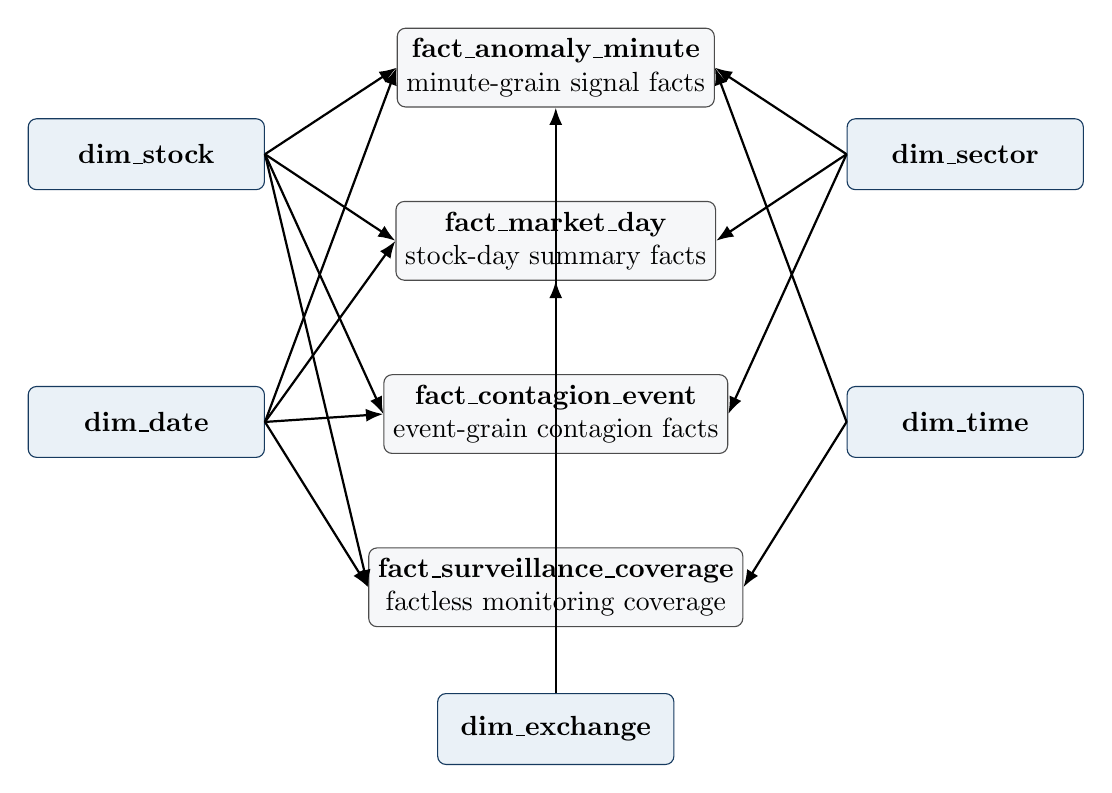
\begin{tikzpicture}[
    dim/.style={draw=accent, rounded corners=3pt, fill=softaccent, minimum width=3cm, minimum height=0.9cm, align=center},
    fact/.style={draw=black!70, rounded corners=3pt, fill=softgray, minimum width=3.6cm, minimum height=1.0cm, align=center},
    arrow/.style={-{Latex[length=2.2mm]}, thick}
]
\node[fact] (minute) at (0,0) {\textbf{fact\_anomaly\_minute}\\minute-grain signal facts};
\node[fact] (day) at (0,-2.2) {\textbf{fact\_market\_day}\\stock-day summary facts};
\node[fact] (contagion) at (0,-4.4) {\textbf{fact\_contagion\_event}\\event-grain contagion facts};
\node[fact] (coverage) at (0,-6.6) {\textbf{fact\_surveillance\_coverage}\\factless monitoring coverage};

\node[dim] (stock) at (-5.2,-1.1) {\textbf{dim\_stock}};
\node[dim] (sector) at (5.2,-1.1) {\textbf{dim\_sector}};
\node[dim] (date) at (-5.2,-4.5) {\textbf{dim\_date}};
\node[dim] (time) at (5.2,-4.5) {\textbf{dim\_time}};
\node[dim] (exchange) at (0,-8.4) {\textbf{dim\_exchange}};

\foreach \target in {minute,day,contagion,coverage}
    \draw[arrow] (stock.east) -- (\target.west);
\foreach \target in {minute,day,contagion}
    \draw[arrow] (sector.west) -- (\target.east);
\foreach \target in {minute,day,contagion,coverage}
    \draw[arrow] (date.east) -- (\target.west);
\foreach \target in {minute,coverage}
    \draw[arrow] (time.west) -- (\target.east);
\foreach \target in {minute,day}
    \draw[arrow] (exchange.north) -- (\target.south);
\end{tikzpicture}
\caption{Warehouse dimensional model}
\label{fig:starschema}
\end{figure}

The dimensions are \texttt{dim\_stock}, \texttt{dim\_sector}, \texttt{dim\_date}, \texttt{dim\_time}, and \texttt{dim\_exchange}. The fact tables are:
\begin{itemize}
    \item \textbf{\texttt{fact\_anomaly\_minute}} at minute grain, keyed by stock, date, and time.
    \item \textbf{\texttt{fact\_market\_day}} at stock-day grain, storing anomaly counts and daily severity summaries.
    \item \textbf{\texttt{fact\_contagion\_event}} at event grain.
    \item \textbf{\texttt{fact\_surveillance\_coverage}} as a factless fact table.
\end{itemize}

The factless coverage table is especially important. During the warm-up period, the anomaly engine is intentionally collecting context without producing scores. If the warehouse only looked at anomaly facts, that time would appear as if the stock had not been monitored at all. Coverage facts fix that gap and make the monitoring story complete.

\subsection{ETL and Non-Volatile Loading}
The ETL service in \path{services/etl/src/etl_service/main.py} is the bridge from operations to analytics. The functions \path{stage_rows}, \path{load_facts}, and \path{run_for_date} implement the warehouse load. The pipeline performs extraction, staging, cleansing, contagion-flag derivation, surrogate key assignment, fact loading, and materialized view refresh. The design is restart-safe: if a load is repeated for the same day, the ETL clears and reloads that date partition rather than silently duplicating rows.

\section{Warehouse Analytics, Querying, and Reporting}
The warehouse exists to support analysis that would be awkward, slow, or semantically unclear on the operational stores. In the current implementation, the warehouse exposes both direct APIs and an analyst-facing query workbench.

\subsection{Materialized Analytical Views}
Several materialized views are prebuilt for common analytical questions:
\begin{itemize}
    \item \texttt{warehouse.mv\_sector\_daily\_summary}
    \item \texttt{warehouse.mv\_sector\_monthly\_summary}
    \item \texttt{warehouse.mv\_sector\_regime\_summary}
    \item \texttt{warehouse.mv\_stock\_signal\_leaders}
    \item \texttt{warehouse.mv\_sector\_momentum\_summary}
    \item \texttt{warehouse.mv\_stock\_persistence\_summary}
    \item \texttt{warehouse.mv\_intraday\_pressure\_profile}
\end{itemize}

These views are not arbitrary extras. They correspond to the kinds of questions an analyst or evaluator is likely to ask: Which sectors were under the most pressure? Which stocks remained persistently abnormal? What part of the trading session concentrated the highest signal intensity? Did contagion cluster around a few names or spread widely?

\subsection{Analyst Query Engine}
The analyst workbench is exposed in the UI as a visual query builder, but it is backed by a deliberately constrained query engine rather than unrestricted SQL execution. The metadata catalog lives in \path{services/api/src/api_service/main.py} in the function \path{_warehouse_query_catalog}. Each dataset declares which dimensions, measures, filters, grouping modes, and sorts are allowed. The API then translates a user selection into a safe SQL statement over warehouse facts or views.

This is an important design choice. It gives the user a BI-like experience without opening the system to arbitrary query strings, accidental full scans, or unstable semantics. The result set can be visualized in the browser, exported as CSV, or printed to PDF through the browser's native print flow.

\subsection{Representative Queries}
The following examples are representative of the analytical work the warehouse supports.

\textbf{1. Sector stress ranking for a trading date}
\begin{verbatim}
SELECT sector_name,
       total_anomalies,
       contagion_event_count,
       peak_daily_composite_score
FROM warehouse.mv_sector_regime_summary
ORDER BY total_anomalies DESC, peak_daily_composite_score DESC
LIMIT 5;
\end{verbatim}

\textbf{2. Persistent high-signal stocks}
\begin{verbatim}
SELECT symbol,
       company_name,
       sector_name,
       anomaly_days,
       total_anomalies,
       anomaly_day_ratio,
       peak_daily_composite_score
FROM warehouse.mv_stock_persistence_summary
ORDER BY anomaly_day_ratio DESC, total_anomalies DESC
LIMIT 10;
\end{verbatim}

\textbf{3. Intraday hotspot analysis}
\begin{verbatim}
SELECT time_label,
       anomaly_minutes,
       distinct_stocks,
       avg_composite_score,
       peak_composite_score
FROM warehouse.mv_intraday_pressure_profile
ORDER BY peak_composite_score DESC
LIMIT 10;
\end{verbatim}

\textbf{4. Fact-level daily summary by sector}
\begin{verbatim}
SELECT d.calendar_date,
       s.sector_name,
       SUM(f.anomaly_count) AS total_anomalies,
       AVG(f.avg_composite_score) AS avg_signal,
       SUM(f.contagion_event_count) AS contagion_events
FROM warehouse.fact_market_day f
JOIN warehouse.dim_date d   ON d.date_sk = f.date_sk
JOIN warehouse.dim_sector s ON s.sector_sk = f.sector_sk
GROUP BY d.calendar_date, s.sector_name
ORDER BY d.calendar_date, total_anomalies DESC;
\end{verbatim}

These queries illustrate why the warehouse is necessary. The operational layer is excellent at ingesting and preserving minute-level events. The warehouse is where those events become analyst-friendly.

\section{Technology Stack and Implementation Details}
The implementation is organized as a monorepo. This turned out to be the right choice for a project with multiple services and shared data contracts. It made it easier to keep the event models, settings, metadata, and helper functions consistent across the collector, engines, ETL, and API.

\begin{table}[H]
\centering
\caption{Technology stack and project role}
\begin{tabularx}{\textwidth}{L{0.2\textwidth}L{0.23\textwidth}Y}
\toprule
\textbf{Layer} & \textbf{Technology} & \textbf{Role in the project} \\
\midrule
Collection & Python, \texttt{yfinance} & Real market data download, captured replay creation, daily hydration, intraday collection \\
Transport & Apache Kafka & Replayable log between collector, storage, and analytics services \\
Operational store & Apache Cassandra & Append-heavy storage for market ticks and anomaly metrics \\
State/cache & Redis & EWMA recovery state, latest market view, latest anomaly view, freshness markers \\
Operational relational store & PostgreSQL & Runs, profiles, daily bars, alerts, contagion events, coverage records \\
Warehouse & PostgreSQL & Dimensions, facts, materialized views, analyst query support \\
Backend API & FastAPI & Unified operational and analytical API surface \\
Frontend & Next.js / React & Operator console, stock workspaces, warehouse UI, analyst studio \\
Deployment & Docker Compose, PowerShell launchers & Reproducible local stack, one-click startup, optional public tunnel \\
\bottomrule
\end{tabularx}
\end{table}

\subsection{Repository Layout}
\begin{table}[H]
\centering
\caption{Key code locations}
\begin{tabularx}{\textwidth}{L{0.31\textwidth}Y}
\toprule
\textbf{Path} & \textbf{Responsibility} \\
\midrule
\path{services/collector/src/collector/main.py} & Collection entry points: daily hydration, capture replay, intraday backfill, normalization, Kafka publish \\
\path{services/storage-consumer/src/storage_consumer/main.py} & Kafka-to-Cassandra persistence for raw market ticks and latest market state \\
\path{services/anomaly-engine/src/anomaly_engine/main.py} & Streaming anomaly scoring, Redis state management, alert emission, anomaly persistence \\
\path{services/contagion-engine/src/contagion_engine/main.py} & Sector contagion windows, event scoring, PostgreSQL persistence \\
\path{services/etl/src/etl_service/main.py} & Staging, cleansing, surrogate key assignment, fact loading, warehouse refresh \\
\path{services/api/src/api_service/main.py} & REST APIs for overview, stocks, contagion, methodology, system health, warehouse analytics, and analyst queries \\
\path{shared/contracts/src/market_surveillance} & Shared models, provider adapters, metadata loaders, history utilities, settings, analytics helpers \\
\path{infra/cassandra/schema.cql} & Cassandra keyspace and table definitions \\
\path{infra/postgres/init.sql} & PostgreSQL schemas, base dimensions, facts, and materialized views \\
\path{infra/postgres/runtime-migrations.sql} & Extended operational tables and advanced warehouse materialized views \\
\path{frontend/app}, \path{frontend/components}, \path{frontend/lib/api.ts} & Page routes, UI components, and frontend data fetching \\
\bottomrule
\end{tabularx}
\end{table}

\subsection{User Interface Surfaces}
The frontend is not just a decorative layer. Each page corresponds to a different kind of question:
\begin{itemize}
    \item \textbf{Overview}: What is happening right now in the monitored intraday universe?
    \item \textbf{Stocks}: Which symbols are listed, hydrated, or currently under intraday coverage?
    \item \textbf{Stock workspace}: What does one symbol look like across daily history, intraday behavior, alerts, and peers?
    \item \textbf{Contagion}: Did sector spillover occur, and if so, how broad was it?
    \item \textbf{Warehouse}: What patterns emerge historically across stocks, sectors, and sessions?
    \item \textbf{Analyst studio}: How can an analyst query the warehouse and export a report without writing SQL directly?
    \item \textbf{Process and Methodology}: How does the pipeline work, and what do the scoring terms mean?
    \item \textbf{System}: Is the stack healthy, current, and internally consistent?
    \item \textbf{Replay}: Which real captured session is being replayed, and what is its current state?
\end{itemize}

\section{Final Demo Plan}
For a presentation, the strongest demo is one that moves from operator value to database value. The recommended flow is:

\begin{enumerate}[leftmargin=1.8em]
    \item Start on the \textbf{Overview} page and explain the distinction between tracked universe, hydrated daily coverage, and intraday loaded symbols.
    \item Use the live tape filters to show that the tape is interactive and backed by real data rather than a static mockup.
    \item Open the alerts panel and explain how anomalies and contagion events become operator-visible items.
    \item Move to \textbf{Stocks}, then open a stock workspace to show daily history, intraday session behavior, anomaly curves, and peer comparison.
    \item Move to \textbf{Contagion} and explain the five-minute observation window and sector propagation logic.
    \item Use \textbf{Process} and \textbf{Methodology} to explain the architectural and mathematical basis of the system.
    \item Move to \textbf{Warehouse} and \textbf{Analyst Studio} to show that the project is not only a stream processor but also a usable analytical system.
    \item End on \textbf{System} to show run history, ETL freshness, row counts, and current scale.
\end{enumerate}

This sequence works well because it tells a story. The audience first sees the problem in operational terms, then sees how the system reasons about it, then sees how the historical layer makes that same data useful for analysts.

\section{Limitations and Future Work}
The system is strong enough for a serious course project, but the honest version of the project still has clear limitations.

First, the current provider configuration uses \texttt{yfinance}. This is acceptable for a real-data-only build and for a defensible demo, but it constrains how much long-horizon intraday depth can be loaded without moving to a broker-grade historical source. The code already includes an \texttt{Upstox} adapter path, but it is not configured in the current deployment and is therefore not claimed as active.

Second, the intraday universe is presently 500 ranked symbols rather than the entire listed exchange. This is a deliberate compromise between breadth, provider limits, and the need to keep the demo fast and honest. The listed-symbol directory still represents the broader market, and daily history coverage is correspondingly wider.

Third, the warehouse is currently populated for one intraday trading day in the loaded replay window. The schema and query engine are designed to support much longer horizons, but the current live facts should be described exactly as they are: analytically meaningful, but not yet multi-month at minute grain.

Fourth, sector coverage in the metadata layer is incomplete. At the time of writing, known-sector coverage is 60.85\%. This does not break the system, but it does mean some symbols remain in an \texttt{Unknown} sector bucket.

Future work is therefore clear:
\begin{itemize}
    \item configure a higher-capability Indian market data provider for broader historical intraday coverage;
    \item extend the ranked intraday universe beyond 500 symbols where provider constraints permit;
    \item improve sector enrichment for the remaining unknown names;
    \item add richer benchmark reporting and workload playback for formal performance evaluation;
    \item enable production-grade notification channels through webhook integrations.
\end{itemize}

\section{Conclusion}
This project began with a simple but demanding requirement: build a system that can treat market surveillance as both a live operational problem and a historical analytical problem. The final implementation meets that requirement by separating the streaming path from the warehouse path without losing the connection between them. Kafka absorbs and replays the stream. Cassandra preserves the operational event log. Redis carries the state that makes fast scoring and fast reads possible. PostgreSQL serves both operational relational needs and long-form analytical work. The ETL process is the disciplined bridge between those worlds.

Just as importantly, the project remains defensible. It does not inflate its claims. It does not rely on synthetic intraday generation. It does not blur the difference between projected scale and actual materialized rows. What it does provide is a coherent, real-data system with a clean architectural story, a usable interface, a warehouse that supports analysis rather than merely storing leftovers, and enough engineering discipline to hold up under questioning.

From the perspective of an Advanced Database Systems course, that is the main contribution of the project. The system is not interesting because it uses many technologies. It is interesting because each storage choice is tied to a workload, each data transformation has a purpose, and the final application shows how distributed ingestion and dimensional analytics can coexist in one carefully designed product.

\end{document}
